\documentclass[15pt]{book}
\usepackage{geometry}                % See geometry.pdf to learn the layout options. There are lots.
\geometry{letterpaper}                   % ... or a4paper or a5paper or ... 
%\geometry{landscape}                % Activate for for rotated page geometry
%\usepackage[parfill]{parskip}    % Activate to begin paragraphs with an empty line rather than an indent
\usepackage{graphicx}
\usepackage{makeidx}
\usepackage{url}

\makeindex

\title{TCH Technology OpenLCB CAN/USB interface}


\author{Written by Tim Hatch}

%\date{}                                           % Activate to display a given date or no date

\begin{document}

\maketitle

\tableofcontents

\chapter{Hardware}
\subsection{Included with purchase}
\begin{itemize}
\item One OpenLCB CAN/USB Interface
\end{itemize}
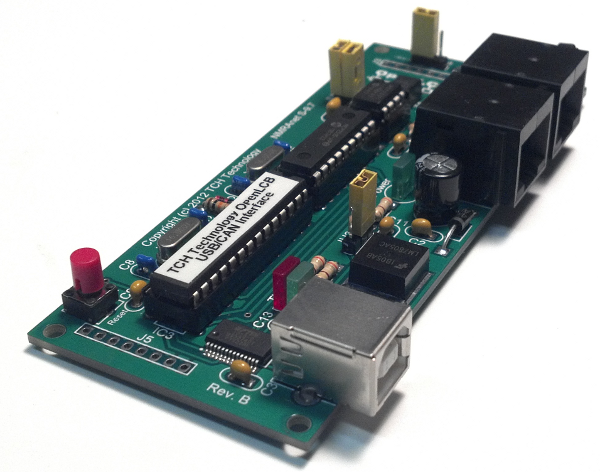
\includegraphics[width=4in]{images/usb_can_a.png}


The TCH Technology CAN/USB interface is used for connecting a computer to an OpenLCB CAN network. The  CAN/USB interface is a plug and play device.  Provisioning is by selection of various jumpers.

\chapter{Provisioning the CAN/USB Interface}

The CAN/USB interface has various jumpers that need to be provisioned before it will work with your computer and other OpenLCB boards.

\section{Powering the CAN/USB Interface}
\index{Power! power, from usb, to usb}
\index{Power! power, from 2.1 mm input}
The TCH Technology CAN/USB can be powered in one of three ways: From an external power supply, via the OpenLCB bus, or via a USB connection from a PC.
\subsection{Power from the external jack}
You may power the CAN/USB using an external power supply that provides a 2.1mm center-positive plug, and between 9 and 12V DC at 500mA or more of current. 
\begin{figure}[htbp]
\begin{center}
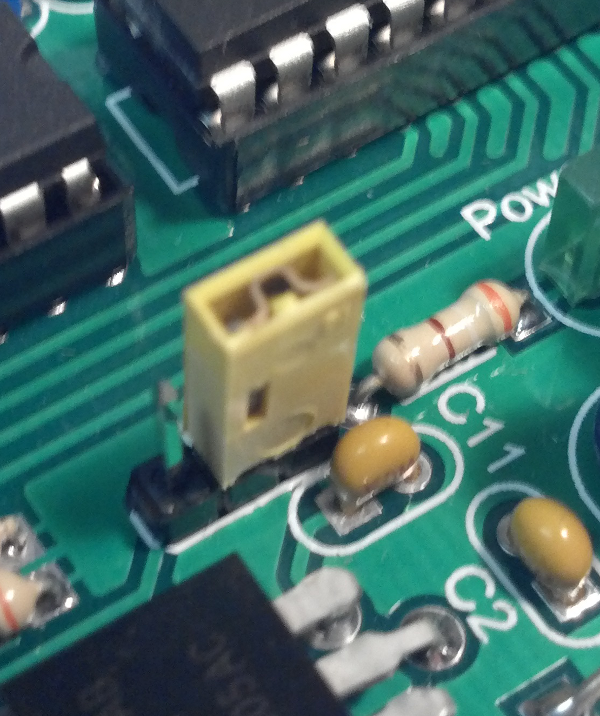
\includegraphics[width=1in]{images/power_line_in.png}
\caption{Jumper set to provide power from line in jack}
\label{CANOUT}
\end{center}
\end{figure}
\subsection{Power from the USB}
Powering the CAN/USB interface from the USB connector.
\begin{figure}[htbp]
\begin{center}
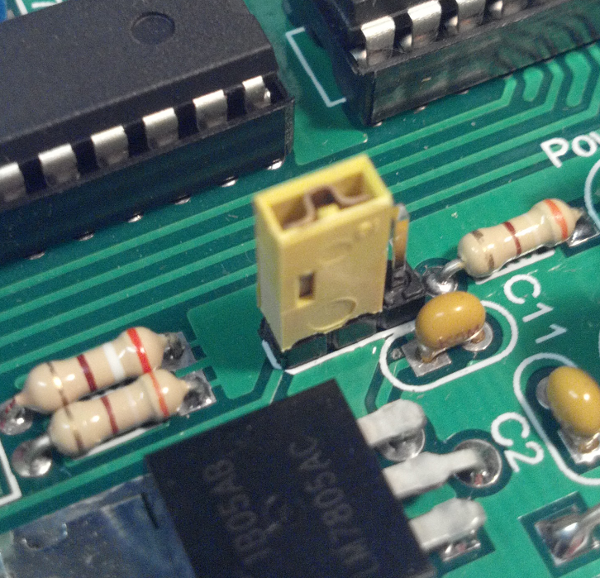
\includegraphics[width=1in]{images/power_line_usb.png}
\caption{Jumper set to provide power from PC USB}
\label{CANOUT}
\end{center}
\end{figure}
\section{Power on the OpenLCB bus}
\index{Power!OpenLCB, to bus}
Note that drawing power from the OpenLCB bus requires that at least one other node be configured to provide power to the OpenLCB bus.
CAN/USB configured to use an external power supply can optionally be configured to provide power to the OpenLCB bus.
\subsection{Provide power to the OpenLCB bus}
\begin{figure}[htbp]
\begin{center}
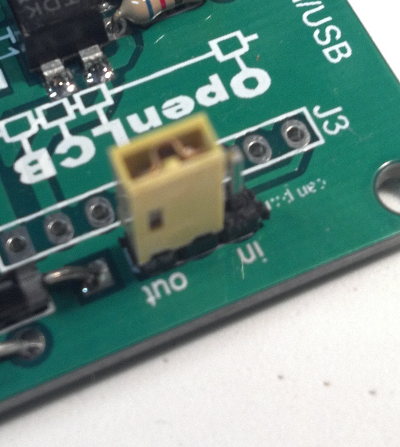
\includegraphics[width=1in]{images/power_out.png}
\caption{CAN POWER jumper set to provide power to the OpenLCB bus}
\label{CANOUT}
\end{center}
\end{figure}
Set the ``can power'' jumper to ``out'', as per \S\ref{CANOUT}.
\subsection{Provide Power from the OpenLCB bus}
\index{Power!OpenLCB, from bus}
\begin{figure}[htbp]
\begin{center}
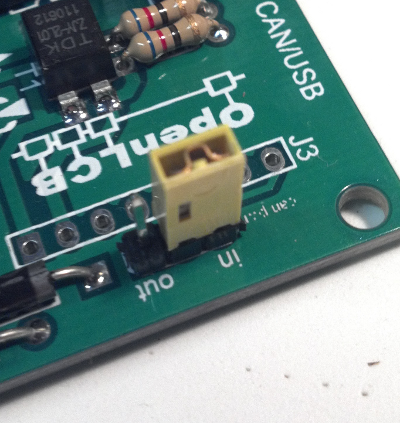
\includegraphics[width=1in]{images/power_in.png}
\caption{CAN POWER jumper set to provide power from the OpenLCB bus}
\label{CANIN}
\end{center}
\end{figure}
Set the ``can power'' jumper to ``in'', as per \S \ref{CANIN}.  Note: Remove the ``can power'' jumper entirely if the CAN/USB will neither draw power from nor provide power to the OpenLCB bus.
\section{Termination of the Bus}
You must determine if you need to teminate your bus.  If your CAN/USB Interface is at the beginning of the CAN bus or at the end of the CAN bus you need to terminate the buss.
\subsection{No termination}
\label{NoTerm}
\index{Termination!None}
To use no termination, the yellow shorting jumers shall be in the non-shorting position. See\S\ref{NoTerm}.
\begin{figure}[htbp]
\begin{center}
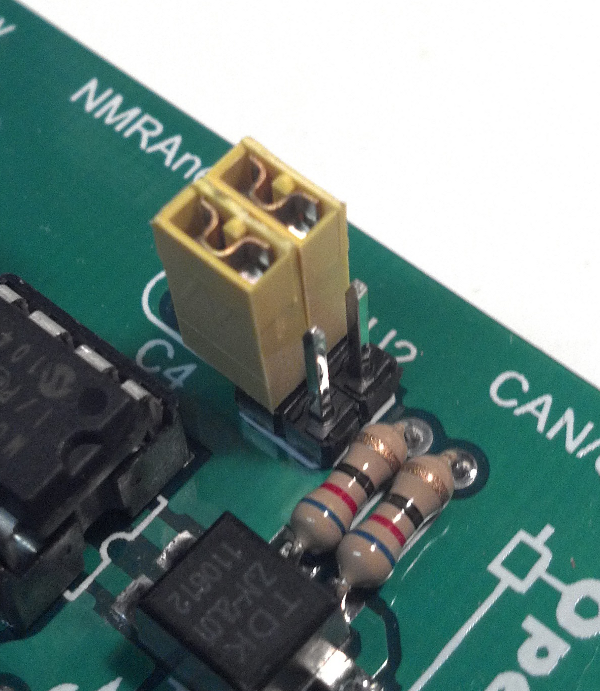
\includegraphics[width=1.5in]{images/term_none.png}
\caption{No termination}
\label{NoTerm}
\end{center}
\end{figure}
\subsection{Resistive termination}
\index{Termination!Resistive}
Resistive termination uses just one yellow shorting jumper set parallel with the two resistors.  See \S\ref{ResTerm}
\begin{figure}[htbp]
\begin{center}
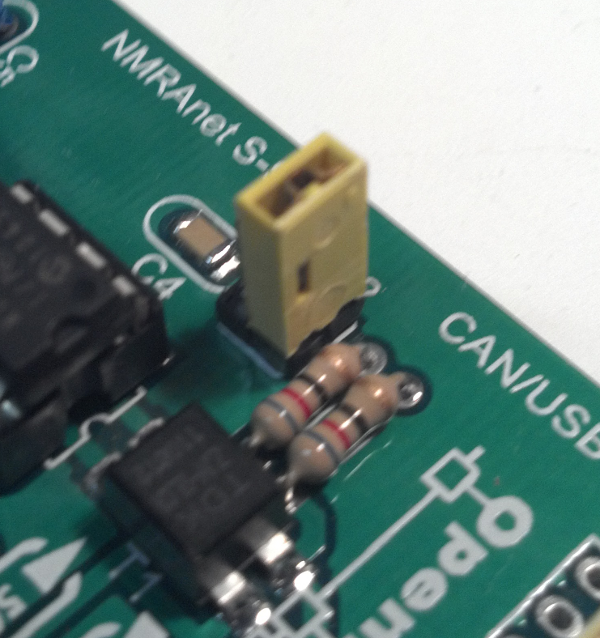
\includegraphics[height=1.5in]{images/term_resistive.png}
\caption{Resistive termination}
\label{ResTerm}
\end{center}
\end{figure}
\subsection{Capacitive termination}
\index{Termination!Capacitive}
Capacitive termination uses two yellow shorting jumpers in parallel.  See\S\ref{CapTerm}
\begin{figure}[htbp]
\begin{center}
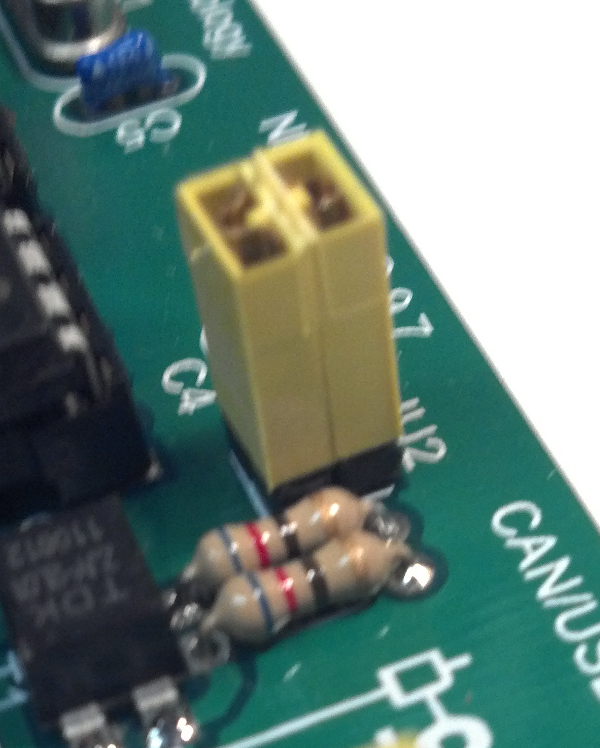
\includegraphics[width=1in]{images/term_capacitive.png}
\caption{Capacitive termination}
\label{CapTerm}
\end{center}
\end{figure}

\section{Baud Rate Selection}
\index{Baud rate!Selection}

The CAN/USB interface has three selections for baud rate speed.  500k baud, 333,333 baud and 230,400 baud.  Selection is done using the yellow jumpers.
\subsection{Proceedure for setting baud rate}
\index{Proceedure!baud rate}

Each time a baud rate is selected, pushing the red reset buton is required to initialize the selection.

\subsection{Default 500k baud}
\index{Baud rate!500k}
For the selection of the default 500k baud there shall be no yellow shorting jumpers on the baud rate selection pin headers.

\subsection{333,333 baud rate selection}
\index{Baud rate!333,333}
Position the yellow shorting jumper as per the figure in \S\ref{333333}
\begin{figure}[htbp]
\begin{center}
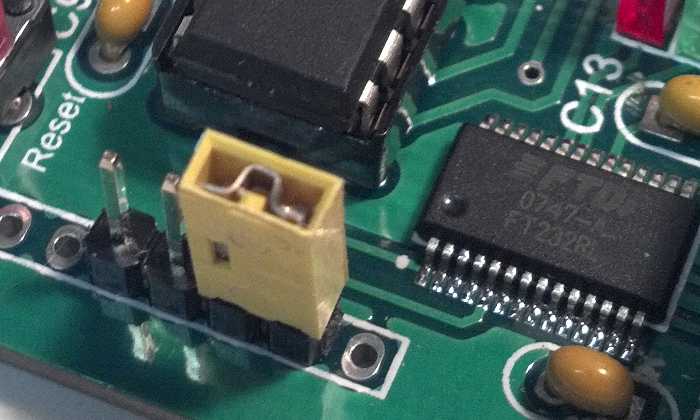
\includegraphics[width=3in]{images/333333_baud.png}
\caption{333,333 baud rate selection}
\label{333333}
\end{center}
\end{figure}


\subsection{230,400 baud rate selection}
\index{Baud rate!230,400}
Position the yellow shorting jumper as per the figure in \S\ref{230400}
\begin{figure}[htbp]
\begin{center}
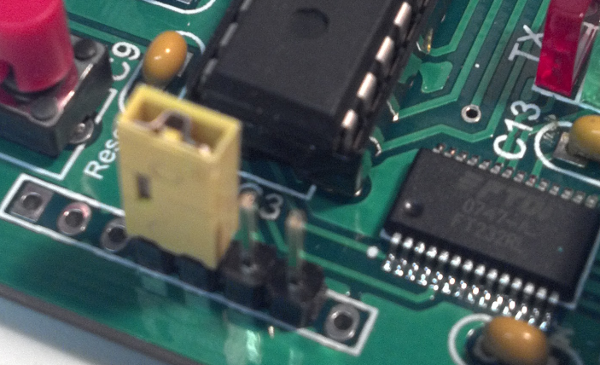
\includegraphics[width=3in]{images/230400_baud.png}
\caption{230,400 baud rate selection}
\label{230400}
\end{center}
\end{figure}

\chapter{Using JMRI Panel Pro}
\index{JMRI! Panel Pro, using}
JMRI Main Screen
\begin{figure}[htbp]
\begin{center}
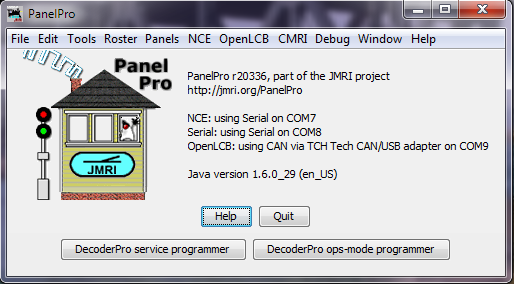
\includegraphics[width=6in]{images/jmri.png}
\caption{JMRI Panel Pro}
\end{center}
\end{figure}

\section{JMRI Preferences}
\subsection{Connections}
JMRI Preferences Screen.  Select OpenLCB for your connection.
\begin{figure}[htbp]
\begin{center}
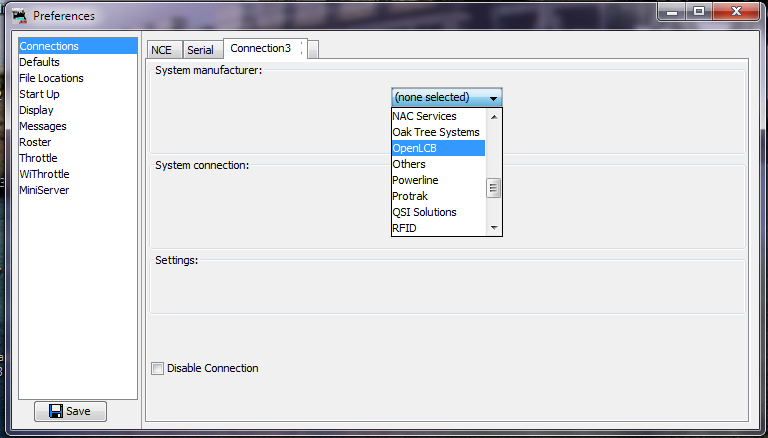
\includegraphics[width=3.5in]{images/jmri_preferences.png}
\caption{JMRI Preferences}
\end{center}
\end{figure}


\subsection{TCH Tech Adapter}
Select the ``CAN via TCH Tech CAN/USB adapter"
\begin{figure}[htbp]
\begin{center}
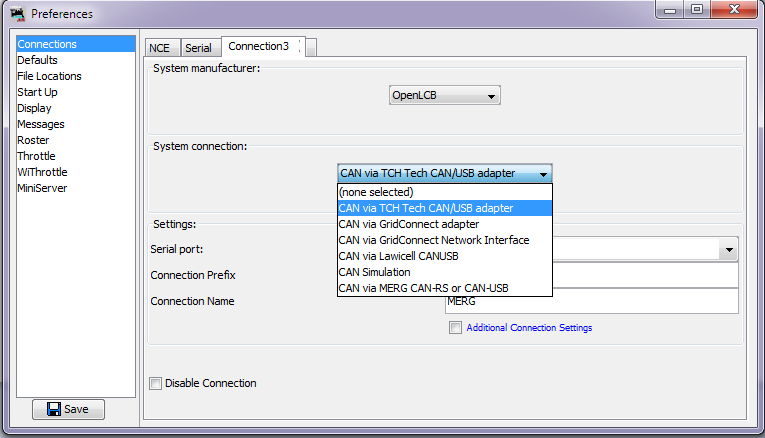
\includegraphics[width=3.5in]{images/jmri_tch_adapter.png}
\caption{JMRI TCH Tech Adapter}
\end{center}
\end{figure}

\subsection{JMRI comport}
Select the ``COM Port"
\begin{figure}[htbp]
\begin{center}
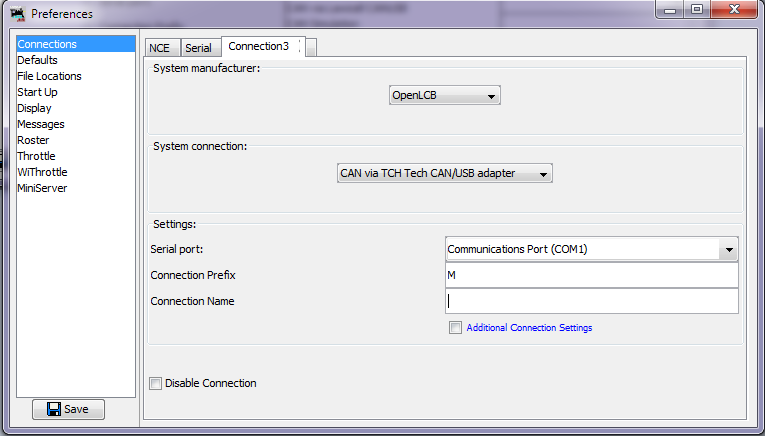
\includegraphics[width=3.5in]{images/jmri_comport.png}
\caption{JMRI comport}
\end{center}
\end{figure}

\subsection{JMRI baud rate }
Type in your ``Connection Name"  usually ``OpenLCB".  Click on the box for Additional Connection Settings. Select the ``comport baud rate"
\begin{figure}[htbp]
\begin{center}
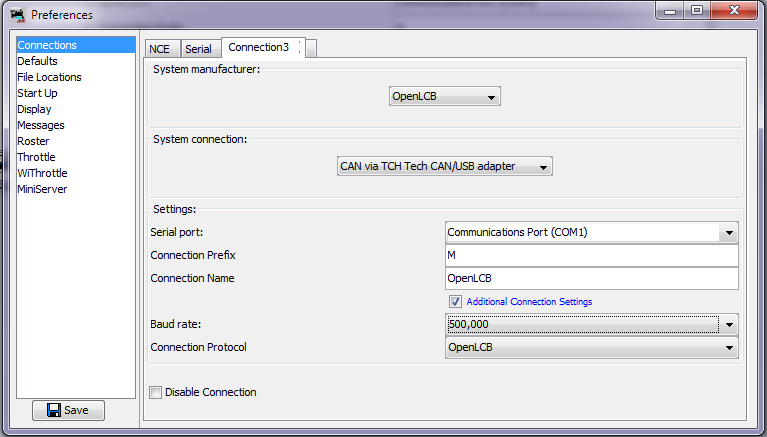
\includegraphics[width=3.5in]{images/baud_rate.png}
\caption{JMRI baud rate selection}
\end{center}
\end{figure}

\subsection{JMRI complete }
Your connection to JMRI should now be complete.
\begin{figure}[htbp]
\begin{center}
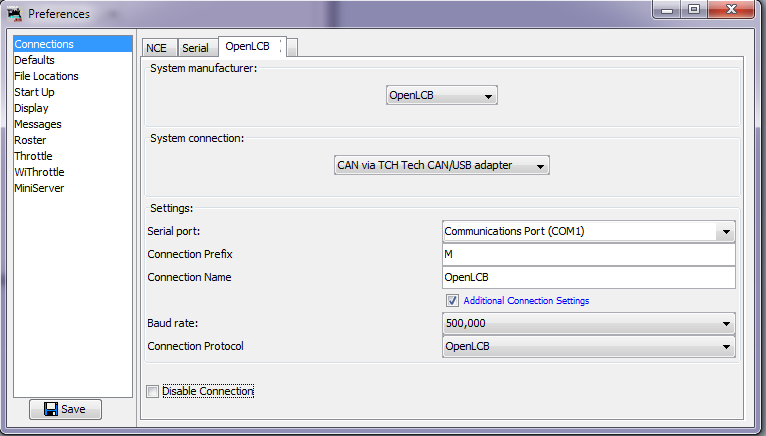
\includegraphics[width=3.5in]{images/jmri_complete.png}
\caption{JMRI Completion}
\end{center}
\end{figure}
%%%%%%%%%%%%%%%%%%%%
%end matters

\printindex

\newpage


 TCH Technology\texttrademark is a trademark of Timothy C. Hatch



\end{document}  